\documentclass{article}
\usepackage[margin=1in]{geometry}
\usepackage{tikz}
\usetikzlibrary{shapes.geometric, arrows, positioning}
%For tikz node diagram setup
\pagenumbering{gobble}

\definecolor{mgreen}{HTML}{689562}
\definecolor{mpurp}{HTML}{85678f}
\definecolor{mblue}{HTML}{3C406C}
\definecolor{mgray}{HTML}{6F6F6F}
\tikzset{trapezium stretches=true}
\tikzstyle{source} = [rectangle, rounded corners, minimum width= 2cm, minimum height = 1cm, text = white, text centered, fill = mgray]
\tikzstyle{input} = [trapezium, trapezium left angle=50, trapezium right angle = 130, minimum width = 1.5cm, minimum height=1cm, text centered, text=white, fill=mgreen]
\tikzstyle{routing} = [diamond, minimum width=2cm, minimum height=1cm, aspect = 2, text width = 2cm, text centered, text=white,fill = mblue]
\tikzstyle{processor} = [rectangle, minimum width = 2cm, minimum height = 1cm, text width = 3cm, text = white, fill = mpurp]
\tikzstyle{cable} = [thick, ->, >=latex]
\tikzstyle{usb} = [thick, <->, >=latex]


\begin{document}
\centering
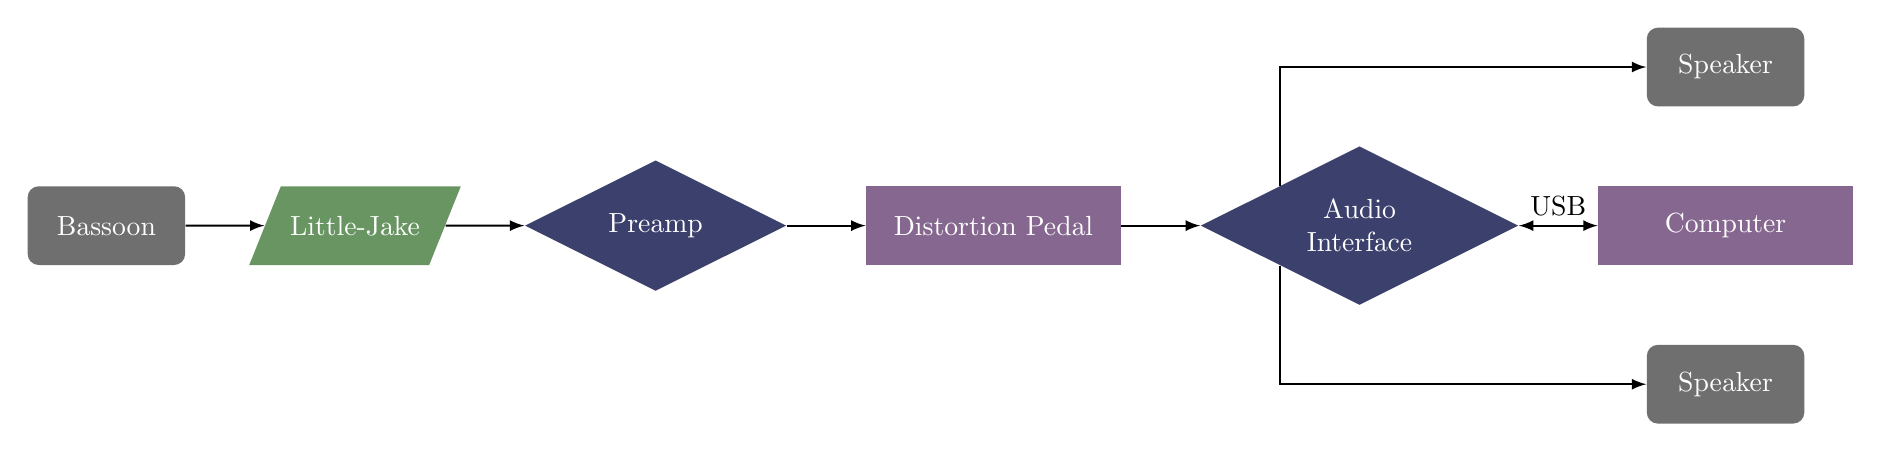
\begin{tikzpicture}[align=center, node distance=1cm]
%Electric Setup
\node (bsn2) [source] {Bassoon};
\node (lj) [input, right = of bsn2] {Little-Jake};
\node (preamp) [routing, right = of lj] {Preamp};
\node (dist) [processor, right = of preamp] {Distortion Pedal};
\node (interface2) [routing, right = of dist] {Audio Interface};
\node (comp2) [processor, text width = 3cm, right = of interface2] {Computer};
\node (speaker3) [source, above = of comp2] {Speaker};
\node (speaker4) [source, below = of comp2] {Speaker};
\draw [cable] (bsn2) -- (lj);
\draw [cable] (lj) -- (preamp);
\draw [cable] (preamp) -- (dist);
\draw [cable] (dist) -- (interface2);
\draw [usb] (interface2) -- node[anchor=south]{USB} (comp2);
\draw [cable] (interface2.north west) |- (speaker3);
\draw [cable] (interface2.south west) |- (speaker4);
\end{tikzpicture}


\end{document}
